\chapter{\exevtitle: extrinsic elastic and viscous anisotropy}

\label{chapter:exev}

The \exevtitle{} software includes routines to compute extrinsic (SPO-related) fabrics and associated elastic and viscous tensors through effective medium theories\\

\section{Effective Medium Theories}

\subsection{Smoothed Transversely Isotropic Long-Wavelength Equivalent (STILWE)}
Introduced by \citep{backus1962jgr}, the STILWE is widely used to estimate the elastic properties of a stack of isotropic layers whose thickness is much smaller than the seismic wavelength. The equivalent elastic moduli of the homogeneous transversely isotropic medium are algebraic combinations of algebraic combinations of two elastic parameters ($\lambda$, $\mu$ or $\theta=Vs^2/Vp^2$). For a VTI medium, the elastic constants can be computed by using averages $\langle \cdot \rangle$ of $\mu$ and $\theta$ as \citep{backus1962jgr}:

\begin{gather}
    A=4(N-S)+R^{-1} (1-2T)^2\\
    C=R^{-1}\\
    F=R^{-1} (1-2T)\\
    L=\langle1/\mu \rangle^{-1}\\
    N=\langle\mu\rangle
\end{gather}

where $R=\langle \theta/\mu \rangle$, $S=\langle \theta\mu \rangle$, $T=\langle \theta \rangle$
The range of $\mu$ and $\theta$ for which the STILWE is stable is $0\leq\theta\leq3/4$ and $0\leq\mu\leq\ +\infty$.\\




\subsection{Differential Effective Medium (DEM) Theory}
The tensorial formulation for DEM is \citep{mclaughlin1977}:

\begin{align}
    \frac{d\mathbf{C^{DEM}}}{dV}&=\frac{1}{1-V}(\mathbf{C}-\mathbf{C^{DEM}})\mathbf{A^i}\\
    \mathbf{A^i}&=[\mathbf{I}+\mathbf{G^s}(\mathbf{C^i}-\mathbf{C^{DEM}} )]^{-1}
\end{align}

where $\mathbf{C^i}$ and $\mathbf{C^{DEM}}$ are the 4th-order elastic tensors of the inclusion and of the effective medium, respectively, $V$ is the volume fraction of the inclusion, $\mathbf{A^i}$ is the ratio of strain inside the inclusion to the strain in the host medium, $\mathbf{I}$ is the symmetric fourth-rank unit tensor, $\mathbf{G^s}$ is the symmetric Green’s interaction tensor \citep{mainprice1997tect},\citep{hornby1994}:

\begin{gather}
    G_{ijkl}^s=\frac{1}{2}(G_{ikjl}+G_{jkil})\\
    G_{ijkl}=\frac{1}{4\pi} \int_{0}^\pi sin(\theta) d\theta \int_{0}^{2\pi} (K_{ij}^{-1}x_k x_l) d\phi 
\end{gather}

Here, the Green’s interaction tensor G depends on the inclusion geometry and matrix elastic tensor through the Christoffel stiffness tensor $K_{ik} (x)=C_{ijkl}^{DEM} x_j x_l$ and directions $x_1=sin\theta cos\phi/a_1$, $x_2=sin\theta sin\phi/a_2$  and $x_3=cos\theta/a_3$, where $a_1$,$a_2$,$a_3$ are the semiaxes of the ellipsoidal inclusion.
Eq. S3.2.1a is solved with a 1st–order in time, 4th-order in space Runge-Kutta method by setting the matrix as the initial effective medium and then by progressively increasing the volume fraction of the inclusion. It is important to note that, for any inclusion concentration, the host medium is always fully interconnected while the inclusions remain isolated.

The DEM solution for an aggregate of spherical inclusions is shown in Fig. \ref{fig:dem_benchmark}, and benchmarked with the analytical solution \citep{mclaughlin1977}:

\begin{center}
$\frac{dK}{dV}=\frac{K-K^{DEM}}{1-V}\frac{K+K^\star}{K^{DEM}+K^\star}$

$\frac{d\mu}{dV}=\frac{\mu-\mu^{DEM}}{1-V}\frac{\mu+\mu^\star}{\mu^{DEM}+\mu^\star}$

where $K^\star=\frac{4}{3}\mu$, $\mu^\star=\frac{1}{6}\mu\frac{9K+8\mu}{K+2\mu}$
\end{center}

\begin{figure}[ht]
    \centering
    \includegraphics[width=1.0\textwidth]{EXEV/DEM_spheres.png}
    \caption{Comparison between analytical and DEM modeling solutions for spherical inclusions}
    \label{fig:dem_benchmark}
\end{figure}


\section{Extrinsic elastic anisotropy}
\label{section:elasticSPO}
Seismic anisotropy can be generated by the strain‐induced lattice preferred orientation (LPO) of minerals with anisotropic elastic properties (as modelled with D-Rex) and/or by the shape‐preferred orientation (SPO) of isotropic compositional heterogeneities. The former anisotropy is referred to as intrinsic mechanical anisotropy, while the latter is referred to as extrinsic mechanical anisotropy. Extrinsic anisotropy occurs when (i) the size of the SPO is much smaller than the wavelength of the seismic signal and (ii) the contrast in isotropic elastic properties between the compositional domains is very large. When these conditions are satisfied, seismology fails to distinguish a finely layered and strongly heterogeneous isotropic medium from a smooth intrinsic anisotropic medium.\\
Within the Earth, extrinsic anisotropy can be related to either (1) the presence of a free gas or liquid phase included in elongated and preferentially oriented grain boundaries, pores, cracks, and porosity bands or (2) grain‐scale (micrometer to centimeter) and/or rock‐scale (centimeter to kilometer) SPO of compositionally distinct domains.\\*
\\
Modelling of extrinsic elastic anisotropy due to SPO is activated with parameter \fonts{spomod} in \texttt{drexs\_input.dat} (when using \drexstitle{})  or \texttt{viztomo\_input.dat} (when using \viztomotitle{}):
\begin{itemize}
    \item[] \fonts{0} = no extrinsic anisotropy is computed, and the original elastic tensor computed as a function of the LPO evolution is retained.
    
    \item[] \fonts{1} = extrinsic elastic anisotropy computed with the STILWE (Smooth Transversely Isotropic Long-Wavelength Equivalent medium; \citep{backus1962jgr}), which calculates the elastic properties for a layered medium with $\geq$ 2 materials. The original elastic tensor computed in \drexmtitle{} is ignored. The newly computed elastic tensor is then rotated with the layering normal to the shortest semiaxis of the FSE (e.g., \citet{olson1984jgr}).
    
    \item[] \fonts{2} = extrinsic elastic anisotropy computed with the DEM (Differential Effective Medium; \citep{mclaughlin1977,mainprice1997tect}), which calculates the elastic properties of a 2-phase matrix-inclusions system. The shape of the inclusions is ellipsoidal and can be defined in \texttt{spo\_input.dat} together with their volume fraction. The elastic tensors of the 2 media are constant and the original elastic tensor computed in \drexmtitle{} is ignored. The inclusions are oriented parallel to $\sigma_1$, the maximum deviatoric stress, and normal to $\sigma_3$, the minimum deviatoric stress, $\pm$ an angle defined by \fonts{phi\_spo}.

    \item[] \fonts{3} = same as \fonts{spomod = 2}, but the elastic tensor computed in \drexmtitle{} is retained for the matrix.
\end{itemize}


In \viztomotitle{} the SPO fabrics are computed for aggregates with ln\textsubscript{fse} $\geq$ \fonts{ln\_fse\_min}, implying that the rocks have accumulated a certain amount of deformation to generate the SPO fabrics. \\
In order to have the possibility to compute seismological synthetics (e.g., SKS-splitting) with the new elastic tensors, these are saved in a \cijkltitle{} file placed in a new directory \fonts{output\_dir}\texttt{/SPO/}.\\

\subsection{STILWE modeling (active when \fonts{spomod = 1})}
The STILWE can be used to model grain-/rock-scale layering when the P-T conditions of each aggregate are known (implying that the geodynamic model is thermo-mechanical and that \fonts{ptmod > 0} when running \drexmtitle, or \drexstitle). Grain-scale or rock-scale layering can be evaluated for 5 lithologies with lookup tables of density and isotropic elastic moduli f(P,T) generated with MMA\_EoS \citep{chust2017jgr}. It is possible to simultaneously compute grain-scale and rock-scale SPO by setting \fonts{spograinmod > 0} and choosing a rock mixture in volfractrock.
When \fonts{ptmod = 0}, the constant C\textsubscript{$\alpha\beta$} of Medium 1 and 2 defined in \texttt{spo\_input.dat} will be used with a relative volume fraction \fonts{Vmax} for Medium 2. \\*
When using the STILWE, the LPO fabrics are ignored.\\*
The SPO modeling parameters to be set in \texttt{spo\_input.dat} are the following:\\
\\
Set type of layered model:
\begin{itemize}
    \item \fonts{spograinmod}: when > 0, computes the grain-scale SPO for a single lithology or lithology mixture as indicated in volfractrock. The allowed lithologies are Harzburgite, Pyrolite, Basalt and Pyroxenite, as Dunite does not generate grain-scale SPO.  The sum of volfractrock must be 100 (\%). It requires \fonts{spomod = 1}, \fonts{ptmod > 0} and \fonts{sporockmod = 0}.
    \item \fonts{sporockmod}: when > 0, computes the rock-scale SPO for the lithology mixture indicated in volfractrock. The sum of volfractrock must be 100 (\%) and there should be $\geq$2 lithologies with volfractrock > 0. It requires \fonts{spomod = 1}, \fonts{ptmod > 0} and \fonts{spograinmod = 0}.
    \item \fonts{volfractrock(1,…,5)}: volume fractions in \% of the 5 different lithologies (\fonts{1}: Dunite; \fonts{2}: Harzburgite; \fonts{3}: Pyrolite; \fonts{4}: Basalt; \fonts{5}: Pyroxenite). The sum must be 100\%.
\end{itemize}

\subsection{DEM modelling (active when \fonts{spomod > 1})}
The presence of a liquid phase (i.e., with null shear modulus) must be always evaluated with the DEM model (\fonts{spomod = 2} or \fonts{3}), as using the STILWE produces infinite elastic anisotropy.\\
As the inclusions are oriented relative to the principal stresses, when using \viztomotitle{} the flow field \textbf{V} from the input \vtptitle{} file needs to be loaded. As such, a copy of the "present-day" \vtptitle{} (where * is given by \fonts{Tend} as defined in \texttt{viztomo\_input.dat}) must be placed in \fonts{cijkl\_dir}.\\
When using the DEM, the matrix elastic tensor can be the constant C\textsubscript{$\alpha\beta$} of Medium 1 (\fonts{spomod = 2}) or the one from the \drexmtitle{} strain-induced LPO modeling (\fonts{spomod = 3}). \\
The inclusions elastic tensor is always given by the constant C\textsubscript{$\alpha\beta$} of Medium 2, and their volume fraction is given either by \fonts{Vmax} or, when \fonts{meltspomod > 0}, by the porosity of the geodynamic model (see Figs. \ref{fig:meltviscosity}, \ref{fig:extrinsic_anisotropy}). \\
The SPO modeling parameters to be set in \texttt{spo\_input.dat} are the following (unless otherwise specified, the variable format is \texttt{double precision}):\\
\\
Assign geodynamic model porosity (valid only when using \viztomotitle{} and not for the single aggregate fabric modelled with \drexstitle):
\begin{itemize}
    \item \fonts{meltspomod}: (Integer) when > 0, it requires an input file from which the porosity distribution in the computational domain is loaded. The inclusions volume fraction is given by the loaded fluid/melt fraction interpolated to the aggregate position.
    \item \fonts{meltfilename}: (String) name of the input HDF5 file with the geodynamic model porosity distribution. This file must be located in \fonts{cijkl\_dir} and can be created with \texttt{/VIZTOMO/makeporosityfile.m}.
\end{itemize}
Set constant elastic tensors (in Voigt notation) and density for the 2 media:
\begin{itemize}
    \item \fonts{Cback}: constant C\textsubscript{$\alpha\beta$} moduli of Medium 1 (Matrix for DEM)
    \item \fonts{Cinc}: constant C\textsubscript{$\alpha\beta$} moduli of Medium 2 (Inclusions for DEM)
\end{itemize}
Set DEM parameters:
\begin{itemize}
    \item \fonts{esa1,esa2,esa3}: define shape of the ellipsoidal inclusions defining the relative length of the 3 semiaxes ( or better to sigma 1, 2, 3). These semiaxes coincide initially with axes 1, 2 and 3 and then rotated such that \fonts{esa1} and \fonts{esa3} are parallel to, respectively, $\sigma_1$ and $\sigma_3$. The aspect ratio should not exceed 1000.
    \item \fonts{Vmax}: maximum inclusions volume fraction ( \fonts{0 < Vmax < 1})
    \item \fonts{Vstp}: volume fraction increments of the inclusions in the DEM model. The larger \fonts{Vstp}, the less accurate is the computation. \fonts{Vstp} should not be larger than 0.01. 
\end{itemize}
Cracks/porosity bands orientation relative to $\sigma_1$:
\begin{itemize}
    \item \fonts{phi\_spo} (\fonts{$\phi\textsubscript{SPO}$}): when different from 0, it allows to rotate around $\sigma_2$ the fluid-filled cracks/porosity bands by an angle  (in $^{\circ}$) with respect to $\sigma_1$ and in the direction of vorticity. As an example, porosity bands in melt-bearing mantle samples forming at relatively large strain are orientated at about $-25^{\circ}$ from $\sigma_1$ during simple shear deformation (the minus sign means that the rotation is against the vorticity) (\citet{katz2006} and references therein).
\end{itemize}



See \ref{table:spo} for the different combinations of SPO model parameters, and Fig \ref{fig:extrinsic_anisotropy} for an application to a 2D oceanic ridge setting.

The program \texttt{/EXEV/DEMelastic/DEMelastic.f90} can be used to compute the two-phase component elastic properties for a range of inclusion ellipsoidal shapes and volume fractions as defined in \texttt{/EXEV/DEMelastic/dem\_input.dat} (\texttt{COMPILE: ./bash\_compile},
 \texttt{RUN: ./demelastic}). \\
The elastic tensors properties saved in file \texttt{elastictensordem.h5} can then be plotted in Flinn diagrams using \texttt{/EXEV/DEMelastic/readDEMelastic.m} (Fig. \ref{fig:dem_elastic}).

\begin{figure}[ht]
    \centering
    \includegraphics[width=0.82\textwidth]{EXEV/dem_elastic0.05.jpg}
    \caption{Flinn diagram showing the elastic properties of an aggregates with $5\%$ in volume of melt-filled ellipsoidal inclusions with different shapes defined by the semiaxes ratios a1/a2 and a2/a3 and matrix-inclusion physical properties as defined in \texttt{dem\_input.dat}. From top to bottom, left to right: P-wave anisotropy, isotropic P-wave anomaly w.r.t. the dry sample, isotropic P- and S-wave velocities, and their ratio.}
    \label{fig:dem_elastic}
\end{figure}

\newpage

\begin{table}[ht]
\centering
\caption{\raggedright Different SPO models as a function of operating mode parameters}
\begin{adjustbox}{width=1\textwidth}
\begin{tabular}{|>{\centering}m{.09\textwidth}|>{\centering}m{0.09\textwidth}|>{\centering}m{0.16\textwidth}|>{\centering}m{0.16\textwidth}|>{\centering}m{0.15\textwidth}|m{0.35\textwidth}|} 

\hline
\fonts{spomod}	& \fonts{ptmod}$^1$	& \fonts{spograinmod} &	\fonts{sporocksmod} &	\fonts{meltspomod}	& Type of model\\ [1ex] 
\hline\hline

 \fonts{1} & \fonts{0} & - & - & - & STILWE with 2 constant C\textsubscript{$\alpha\beta$} from \texttt{spo\_input.dat} \\\hline

\fonts{1} &	\fonts{1} & \fonts{1} & \fonts{0} & - & \small{STILWE with grain-scale SPO f(P,T)} \\\hline
\fonts{1} & \fonts{1} & \fonts{0} & \fonts{1} & - & STILWE with rock-scale SPO f(P,T)\\\hline
\fonts{2} & - & - & - & \fonts{0} & DEM with constant C\textsubscript{$\alpha\beta$}, ellipsoidal shape and $\psi^2$ = \fonts{Vmax} from \texttt{spo\_input.dat} \\\hline
\fonts{2} & - & - & - & \fonts{1} & DEM with constant C\textsubscript{$\alpha\beta$} and ellipsoidal shape from \texttt{spo\_input.dat}. $\psi$ from geodynamic model\\\hline
\fonts{3} & - & - & - & \fonts{0} & DEM with C\textsubscript{$\alpha\beta$} from LPO for matrix, while constant C\textsubscript{$\alpha\beta$} for inclusions, ellipsoid shape and $\psi$ = \fonts{Vmax} defined in \texttt{spo\_input.dat}\\\hline
\fonts{3} & - & - & - & \fonts{1} & DEM with C\textsubscript{$\alpha\beta$} from LPO for matrix, while constant C\textsubscript{$\alpha\beta$} for inclusions, ellipsoid shape defined in \texttt{spo\_input.dat}. $\psi$ from geodynamic model\\
\hline
\hline

\end{tabular}

\end{adjustbox}

\raggedright \footnotesize{$^1$ to be set in the \texttt{drexs\_input.dat} or \texttt{viztomo\_input.dat} files.}\\
\raggedright \footnotesize{$^2$ porosity.}\\
\vspace{0.3cm}

\raggedright \footnotesize{The '-' symbol means that the corresponding parameter is ignored}


\label{table:spo}
\end{table}

\newpage

\section{Extrinsic viscous anisotropy}
The modelling of extrinsic viscous anisotropy related to rock-scale and grain-scale fabrics relies on the DEM modelling and a geometric parametrization extrapolated from 3D high-resolution simulations of deforming matrix-inclusions aggregates \citep{demontserrat2021}. \\
The DEM modelling is used to generate a database of viscous tensors for different matrix-inclusions viscosity contrasts, relative volume fraction and inclusions aspect ratios. Given the aggregate bulk FSE, the geometric parametrization provides an estimate of the inclusions average aspect ratio and orientation, thus allowing the mapping of the viscous tensor from the database and its rotation with respect to the FSE axes orientation. \\
Thus, the first modelling phase requires generating the DEM database (stored in file \texttt{viscoustensordem.h5}), which, together with the geometric parametrization, can be then exploited to estimate the local viscous tensor due to SPO-related fabrics in every point of the computational domain. The viscous tensor can be returned on the fly when the proper functions are called from a running geodynamic model (coupled mechanical simulations). Alternatively, its anisotropic properties can be computed for post-processing visualization (uncoupled mechanical simulations).\\
It is important to note that the values of the aggregate viscous tensor are always normalized with respect to the isotropic matrix viscosity $\eta_{mat}$. Hence, to retrieve the total viscous tensor:

$\pmb{\eta_{tot}}= \pmb{\eta_{DEM}}\cdot\eta_{mat}$


\subsection{Generate the viscous tensor database}
\label{section:viscousDEM}

The main file \texttt{DEMviscous.f90} can be compiled and run as:

\texttt{DIRECTORY: /EXEV/DEMviscous}\\*
\\
\texttt{COMPILE: ./bash\_compile}\\*
\\
\texttt{RUN: ./demviscous}\\*

The DEM modeling parameters to be set in the parameter input file \texttt{dem\_input.dat} are the following (unless otherwise specified, the variable format is \texttt{double precision}):
\begin{itemize}
    \item \fonts{devmod}: (Integer) 
    \begin{itemize}
        \item[] \fonts{0} = compute total viscous tensor
        \item[] \fonts{>0} = compute deviatoric viscous tensor
    \end{itemize}
\end{itemize}

Set viscosities for the 2 media:
\begin{itemize}

    \item \fonts{isotropicmod}: (Integer)  
    \begin{itemize}
        \item[] \fonts{0} = viscous tensors as defined in Voigt notation by \pmb{$\eta_{mat}$} and \pmb{$\eta_{inc}$}
        \item[] \fonts{>0} = force the viscous tensors to be isotropic with the range of viscosity contrasts defined by \fonts{etacontrmin}, \fonts{etacontrmax}, \fonts{etacontrstp}
    \end{itemize}
    \item \fonts{etacontrlogscalemod}: (Integer), when > 0, the following viscosity contrasts must be defined as $log_{10}$.
    \item \fonts{etacontrmin}, \fonts{etacontrmax}, \fonts{etacontrstp}: define min, max and increment of isotropic viscosity contrasts.
    
    \item \pmb{$\eta_{mat}$}: $\eta_{\alpha\beta}$ moduli of Medium 1 (Matrix for DEM)
    \item \pmb{$\eta_{inc}$}: $\eta_{\alpha\beta}$ moduli of Medium 2 (Inclusions for DEM)

\end{itemize}

Define inclusions shape range:
\begin{itemize}
    \item \fonts{axislogscalemod}: (Integer), when > 0, the following semiaxes lengths must be defined as $log_{10}$.
    \item \fonts{esa1,esa2,esa3}: define shape of the ellipsoidal inclusions defining the range of lengths for, respectively, the maximum, intermediate, minimum semiaxes normalized to that of the smallest one. Thus, \fonts{esa3}, the length of semiaxis 3, should be always 1. The range of lengths should be given as the min. max. and increment lengths.
\end{itemize}
    
Define array of inclusions volume fraction for which the viscous tensor is saved:
\begin{itemize}
    \item \fonts{Volsavemin}: minimum inclusions volume fraction ( \fonts{0 < Volsavemin < Vsavemax}). It must be a multiple of \fonts{Vstpdem}.
    \item \fonts{Volsavemax}: maximum inclusions volume fraction ( \fonts{Volsavemin < Volsavemax < 1}). It must be a multiple of \fonts{Vstpdem}.
    \item \fonts{Volsavestp}: volume fraction increments of the inclusions in the DEM model. It must be a multiple of \fonts{Vstpdem}. 
\end{itemize}

Set volume fraction increment for DEM solution
\begin{itemize}
    \item \fonts{Vstpdem}: it is recommended to keep it as low as possible, especially for large aspect ratios, as the larger \fonts{Vstpdem}, the less accurate is the computation. However, bear in mind that the smallest the volume increment, the larger the number of iterations and the longer the computational time. As a rule of thumb, \fonts{Vstpdem} should not be larger than 0.01, and a good choice is 0.005.
\end{itemize}

The viscous tensor database is saved in the output file \texttt{EXEV/DEMviscous/viscoustensordem.h5} that must be then copied/moved in the \vizvisctitle{} directory.

The viscous tensors properties saved in file \texttt{viscoustensordem.h5} can then be plotted in Flinn diagrams using \texttt{/EXEV/DEMviscous/readDEMviscous.m}.

\\
In \texttt{VIZVISC/viscoustensordem.h5} we provide such a database for deviatoric viscous tensors that can be readily used and computed in the parameter ranges:\\* 
\\
$log_{10}(etac)=-3:1:3$,\\
$log_{10}(esa1)=0:0.1:3$,\\
$log_{10}(esa2)=0:0.1:3$,\\
$log_{10}(esa3)=0$,\\
$Volume fraction = 0.05:0.05:0.3$.
\vfill{}

\subsection{Coupled mechanical simulations}

\texttt{DIRECTORY: /EXEV}\\*

In order to update the \textbf{F} tensor and extract the associated \pmb{$\eta$} tensor from the database, the file \texttt{viscoustensor.f90} must be compiled together with \texttt{moduledem.f90}. This file includes subroutine \texttt{viscoustensor()} to be called from the large-scale geodynamic model by inputting the following variables:

\begin{itemize}
    \item[] \fonts{x1m} = axis 1 coordinate. In polar coordinates, longitude in radians (double)
    \item[] \fonts{x3m} = axis 3 coordinate. In polar coordinates, colatitude in radians (double). In 2D cylindrical/annulus, set to pi/2.0 
    \item[] \fonts{cartspher} = cartesian (1) or polar (2) domain (integer)
    \item[] \fonts{yinyang} = Yin-Yang grid for 3D global simulations, active when = 2 (integer)
    \item[] \fonts{fse0} = particle Fij (3x3 double) in cartesian coordinates       
    \item[] \fonts{l} = particle velocity gradient (3x3 double) in cartesian coordinates
    \item[] \fonts{dt} = timestep (double)                
    \item[] \fonts{etac} = matrix-inclusions isotropic viscosity contrast: $\eta_inc/\eta_mat$ (double). For hard inclusions (\fonts{etac} $ > 1$), allowed values are \fonts{etac}$ = 10, 100, 1000$
    \item[] \fonts{volinc} = inclusions volume fraction (double). Allowed values are \fonts{volinc} $= 0.1, 0.2, 0.3$.
\end{itemize}

The function returns as an output:
\begin{itemize}
    \item[] \fonts{fse}  = updated particle \textbf{F} tensor (3x3 double) in cartesian coordinates      
    \item[] \fonts{etavoigt} = mapped viscous tensor (6x6 double)
\end{itemize}


\vfill{}

\subsection{Uncoupled mechanical simulations: visualizing the viscous tensors with \vizvisctitle{}}

\texttt{DIRECTORY: /VIZVISC}\\*
\\
\texttt{COMPILE: ./bash\_compile}\\*
\\
\texttt{RUN: ./vizvisc vizvisc\_input.dat}\\*

\vizvisctitle{} is a software pretty much similar to \viztomotitle{}. It includes routines for post-processing the \cijkltitle{} output files generated with \drexmtitle{} and for visualizing the \pmb{$\eta$} anisotropy and \textbf{FSE} tensors with \paraviewtitle{}. The viscous tensor \pmb{$\eta$} due to extrinsic viscous anisotropy is extracted from a database of tensors according to the FSE geometry, the matrix-inclusions viscosity contrast (\fonts{etac}) and the inclusions volume fraction (\fonts{volinc}). Thus, pre-computation of the viscous tensor database as explained in section \ref{section:viscousDEM} is required before running \vizvisctitle{} (or one can use the one provided as explained above). The viscous anisotropy is visualized on an eulerian grid defined below, as a function of the radial and azimuthal viscous anisotropy (which are analogous to those defined for elastic anisotropy) computed in the FSE reference frame.

The parameter input file is \texttt{vizvisc\_input.dat}, where the following parameters can be set (unless otherwise specified, the variable format is \texttt{double precision}): 

A) Input and output directories/files
\begin{itemize}
    \item \fonts{cijkl\_dir}: (String) path to input directory where to load the \drexmtitle{} \cijkltitle{} output files (the path should end with  “/” )
	\item \fonts{output\_dir}: (String) path to output directory where to save the visualization output (the path should end with  “/” ), which can be or not the same as \fonts{cijkl\_dir}
	\item \fonts{Tinit},\fonts{Tstep},\fonts{Tend}: (Integers) initial, increment and final number of input \cijkltitle{} files to be processed. When \fonts{Tinit} = \fonts{Tend}, only a single \cijkltitle{} file is processed.
\end{itemize}

B) Define viscosity contrast and inclusions volume fraction
\begin{itemize}
    \item \fonts{etac}: isotropic viscosity contrast: $\eta_{inc}/\eta_{mat}$. For hard inclusions (\fonts{etac} $ > 1$), allowed values are \fonts{etac}$ = 10, 100, 1000$ 
	\item \fonts{volinc}: inclusions volume fraction. Allowed values are \fonts{volinc} $= 0.1, 0.2, 0.3$.
\end{itemize}

C) Visualize properties of Lagrangian aggregates:
\begin{itemize}
    
    \item \fonts{Lagrangian}: (Integer) when > 0, activates visualization of Lagrangian aggregates. The datasets saved in file \texttt{lagrangian*.h5} can be loaded on PARAVIEW with the corresponding file \texttt{XDMF.lagrangian*.xmf}. Vectors can be visualized applying the Glyph filter
	
	\item \fonts{ln\_fse\_min}: assumes values >= 0.0, and indicates the threshold of\\ ln\textsubscript{fse} = ln(fse\textsubscript{max}/fse\textsubscript{min}) above which aggregates properties are visualized. It allows to skip aggregates that experienced low deformation and are nearly isotropic (try with 0.5, for example, as suggested by \citet{becker2006epsl}). When  = 0.0, all aggregates are displayed.
	
	\item \fonts{uppermantlemod}: (Integer) when > 0, displays only upper mantle aggregates.
	
	\item \fonts{rocktypemod}: (Integer) when > 0, displays the rocktype of the aggregates.
	
	\item \fonts{fse3Dmod}\footnotemark: (Integer) when > 0, the left stretch tensor \textbf{FSE} of ALL aggregates are saved in file \texttt{3Dfse*.h5}, and can be loaded on \paraviewtitle{} with \texttt{XDMF.3Dfse*.xmf}. Applying the TensorGlyph filter, the 3D FSE are displayed. The ellipsoids can be colored according to the rocktype or fse\textsubscript{max} (suggestion: set the scale factor equal to the initial spacing of the aggregates defined in \texttt{drexm\_input.dat}) (see Fig. \ref{fig:polarcells_viscous}C).
	
	\item \fonts{fseminmod}: (Integer) when > 0, saves the fse\textsubscript{min} vector scaled by ln\textsubscript{fse}.
	
	\item \fonts{fsemaxmod}: (Integer) when > 0, saves the fse\textsubscript{max} vector scaled by ln\textsubscript{fse}.
	
\end{itemize}

\footnotetext{Visualizing the 3D ellipsoid requires lots of computer memory, so be careful!}

D) Eulerian gridding: interpolate the \pmb{$\eta$} and \textbf{FSE} tensors of Lagrangian crystal aggregates to an Eulerian grid and visualize the anisotorpic properties of \pmb{$\eta$} at each grid node only when ln\textsubscript{fse NODE} > \fonts{ln\_fse\_min}.

\begin{itemize}
    \item \fonts{Eulerian}: (Integer) when > 0, activates Eulerian gridding and visualization of Eulerian nodes elastic properties. The datasets saved in files named \texttt{eulerian*.h5} can be loaded on PARAVIEW with the corresponding files \texttt{XDMF.eulerian*.xmf}.

	\item \fonts{n1first},\fonts{n1last},\fonts{nx11}: define Eulerian grid axis 1: min, max coordinates (in $m$ or $m'$ in cartesian coord.; in degrees in polar/spherical coord.), number of nodes (2 $\leq$ Integer $\leq$ number of aggregates along axis 1).  
	\item \fonts{n2first},\fonts{n2last},\fonts{nx21}: define Eulerian grid axis 2: min, max coordinates, number of nodes (2 $\leq$ Integer $\leq$ number of aggregates along axis 2).  
	\item \fonts{n3first},\fonts{n3last},\fonts{nx31}: define Eulerian grid axis 3: min, max coordinates (in $m$ or $m'$ in cartesian coord.; in degrees in spherical coord.), number of nodes (2 $\leq$ Integer $\leq$ number of aggregates along axis 3).  
	
	\item \fonts{radialmod}: (Integer) compute the radial anisotropy as a scalar when ln\textsubscript{fse NODE} > \fonts{ln\_fse\_min}:

    \begin{itemize}
        \item[] \fonts{0} = no radial anisotropy
        \item[] \fonts{1} = radial anisotropy computed as $\xi=N/L$
        \item[] \fonts{2} = radial anisotropy computed as $\xi(\%)=\sqrt{(N/L)-1}\cdot100$
    \end{itemize}
    where
    $N=\frac{1}{8} (\eta_{11}+\eta_{22} )-\frac{1}{4} \eta_{12}+\frac{1}{2} \eta_{66}$,
    $L=\frac{1}{2} (\eta_{44}+\eta_{55})$
    
	\item \fonts{azimod}: (Integer) compute the azimuthal anisotropy when ln\textsubscript{fse NODE} > \fonts{ln\_fse\_min}. In 2D, only the magnitude G of the azimuthal anisotropy is saved. In 3D, it is possible to visualize also the azimuth of the fast V\textsubscript{SV} indicated by a vector that can be plotted with the Glyph filter of \paraviewtitle{}. The 3D vector is scaled by G, and saved in files \texttt{XDMF.azianis*.xmf} and \texttt{azianis*.h5}.

    \begin{itemize}
        \item[] \fonts{0} = no azimuthal anisotropy
        \item[] \fonts{1} = azimutahl anisotropy computed as $G=\sqrt{{G_C}^2+{G_S}^2} $ 
        \item[] \fonts{2} = azimutahl anisotropy computed as $G(\%)=\sqrt{\eta_{55}/\eta_{44} )-1}\cdot100$
    \end{itemize}
    where $G_C=\frac{1}{2}(\eta_{55}-\eta_{44} )  ; G_S=\eta_{54}$
	
	\item \fonts{aziscalex1}, \fonts{aziscalex2}, \fonts{aziscalex3}: set position of scale bar for azimuthal anisotropy in 3D models (in $m$ or $m'$ in cartesian coord.; in degrees in polar/spherical coord. for \fonts{aziscalex1} and, in 3D, \fonts{aziscalex3}). The bar length correspond to G = 1\% and it is oriented parallel to x1 axis. 
	
\end{itemize}

\vspace{1cm}

Figure \ref{fig:polarcells_viscous} shows the viscous anisotropy in the FSE reference frame for the steady-state global scale convection model in 2D polar coordinates explained in section \ref{section:cookbook_2Dconvection}. \\
The run can be executed after having computed the velocity field with \texttt{cartesiancells.m} (that returns file \texttt{vtp0001.h5}), and the \textbf{F} field with \drexmtitle{} (that returns file \texttt{Cijkl0001.h5}), as:

\texttt{RUN:./vizvisc ../cookbooks/2Dpolar\_convection/vizvisc\_input.dat}\\*

For the other examples shown in the cookbooks chapter, it is straightforward to prepare the input file \texttt{vizvisc\_input.dat}, with several parameters similar to those found in \texttt{viztomo\_input.dat}.

\begin{figure}[ht]
    \centering
    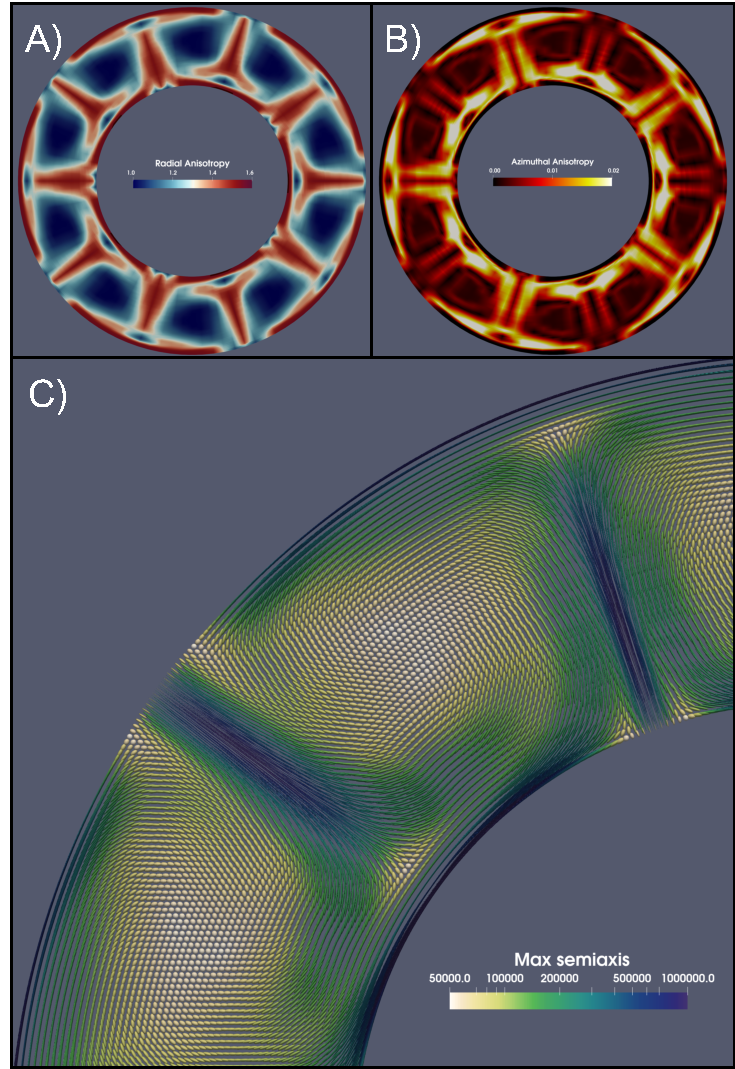
\includegraphics{EXEV/polarcells_viscous_composition.pdf}
    \caption{Steady-state  convection  patterns  in  polar  coordinates  created  with \texttt{polarcells.m}.  A) Radial and B) Azimuthal viscous anisotropy when $\fonts{etac}=0.1$ and $\fonts{volinc}=0.2$; C) the shape and orientation of the FSE ellipsoids plotted with the \paraviewtitle{} tool TensorGlyph. The ellipsoids are color-coded according to the length of the maximum semiaxis upscaled by 50 km.\\
    }
    \label{fig:polarcells_viscous}
\end{figure}

\vfill % Fill the rest of the page with whitespace

\vfill{}

\newpage

